\part{SİMÜLASYON MODELİ}
\thispagestyle{empty}
\newpage
\section{YENİLENEBİLİR ENERJİ SİSTEMLERİNDE KULLANILAN ALGILAYICILARIN VERİ YAPILARI}

Enerji sistemlerindeki veri transfer standartlarını oluşturabilmek için \gls{iec} 61850 iletişim standardı oluşturulmuştur. Bu standart sayesinde enerji santrallerinde oluşturulan veriler sayesinde kontrol, gözlem ve enerji sistemlerinde oluşabilecek arızaların canlı bir şekilde kontrolünün sağlanması amaçlanmıştır \cite{1385190}. Bu tez çalışmasında bahsedildiği üzere Rüzgar enerji türbinleri ve güneş enerji panellerinde oluşturulacak sistemsel çalışma verilerinin aktif bir şekilde kontrolü amaçlandu. Bu kontrolün sağlanması için \gls{iec} 61850 ve benzer standartlardan olan 61400-25 standartları dikkate alınmıştır \cite{Olsen_prototypeof} \cite{francisco2016protection}.


\subsection{Rüzgar Enerji Sistemlerinde Veri Yapıları}
Rüzgar enerji türbinleri ile kontrol odası arasındaki iletişim sistemi, enerji üretimi işini yüklenen firmalar tarafından belirli bir standarda bağlı olmadan gözlem sistemleri bulunmaktadır. Bu durum yüklenici firmaların hepsinde kendisine özel bir çözüm oluşturmaya sebebiyet vermiştir. Bu sorunu açıklamak için, Danimarkalı büyük bir türbin firması ilgili haberleşme çözümü için \gls{iec}'ye başvuruda bulunması sonrası \gls{iec} 61400 standardı geliştirilmiş oldu \cite{Olsen_prototypeof}.

\gls{iec} 61400-25 standardı, rüzgar enerjisi santrallerinin izlenmesi ve kontrolü için birleşik bir iletişimin tanımlanması ve standartlaştırılması için özel bir versiyondur. \gls{iec} 61400-25 serisi, genel olarak trafo merkezlerindeki iletişim ağlarını ve sistemleri tanımla-yan \gls{iec} 61850 serisi standartların bir uzantısıdır. 


\gls{iec} 61400-25 standardı sayesinde, enerji üretim sistemindeki algılayıcılardan oluşan veriler dijital haberleşme standartlarında tekrardan yapılandırılıp komuta kontrol merkezlerine iletilir. İlgili standarda ait 6 alt kategoride veri iletişim standardı yayınlandı.

•	Genel tanımlar ilkeler ve modeller (\gls{iec} 61400-25-1).

•	Rüzgar türbinlerinin enformasyon model standardı (\gls{iec} 61400-25-2).

•	Enformasyon değişim model standardı (\gls{iec} 61400-25-3).

•	İletişim profilinde eşleme standardı (\gls{iec} 61400-25-4).

•	Rüzgar enerji santrallerinde izleme ve kontrol altyapısının uygunluk testleri (\gls{iec} 61400-25-5).

Rüzgar enerji santrallerindeki kontrol ve durum raporu için çalışan mantıksal düğümlerin veri sınıflandırılması \cite{Olsen_prototypeof}.

\subsection{\gls{iec} 61400-25-2 Standardı}

Enformasyon modeli standardı sayesinde rüzgar enerji santrallerinin faaliyeti sırasında yapılan ölçüm ve durum değerleri veri iletişimine hazır hale getirilir. Buna göre enerji santralinde kullanılan tüm donanımlara ait bir veri yapısı oluşturulur. \gls{iec} 61850 standardına göre belirtilen veri haberleşme standardıyla birlikte 61400-25 standardı birlikte incelendiğinde, bir rüzgar enerji türbininde üretilen veriler dokuz adet farklı modülde toplanmaktadır. İlgili modüllerin kısaltması Şekil \ref{fig:figure15}’de gösterilmiştir. Tablo \ref{tab:tabb2}’de türbin içi modüllerin açıklaması ve sensör sayıları gösterilmiştir \cite{francisco2016protection}\cite{trinnass}\cite{san2007use}.



\begin{figure}[htbp]
\centerline{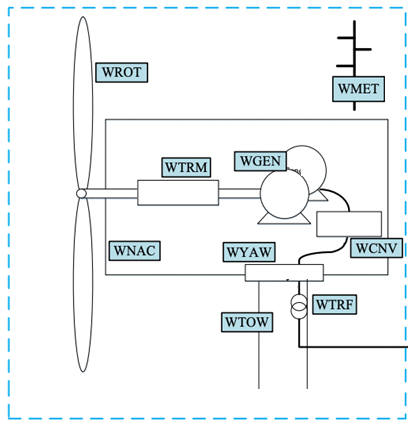
\includegraphics[width=\columnwidth]{Resim/Sekil4-1.png}}
\caption{Türbin içi mantıksal düğümler(\protect\citeA{jannasch2009daten}).}
\label{fig:figure15}
\end{figure}

\gls{iec} 61850 ve \gls{iec} 61400 standartları dikkate alındığında bir rüzgar türbininin sağlıklı bir şekilde çalışması için üzerinde faal durumda olması gereken yetmiş doksan analog, otuz iki adet durum algılayıcısı bulunmalıdır. Tablo \ref{tab:tabb2}’de bir rüzgar türbininde bulunan algılayıcıların sayıları ve bağlı oldukları modüller gösterilmiştir. Tablo \ref{tab:WNACdetay}’de türbin içi modüllerden \gls{wnac}, rüzgar türbinlerinin pal kısmını kapsayan motor mekanizmasına ait modüldür. Şekil \ref{fig:figure15}’den kapsadığı bölge gözlemlenebilir. Bu modüle ait 4 adet durum algılayıcısı ve 11 adet analog algılayıcı bulunmaktadır. Algılayıcıların tanımı Tablo \ref{tab:WNACdetay}’de gösterilmiştir. 
\cite{francisco2016protection}\cite{trinnass}\cite{san2007use}.


\begin{table}[htbp]
\centering
\caption{Türbin içi mantıksal düğüm özellikleri}
\label{tab:tabb2}
\begin{tabular}{ccccc}
\begin{tabular}[c]{@{}c@{}}Modül\\ İsmi\end{tabular} &
  \begin{tabular}[c]{@{}c@{}}Modül\\ Tanımı\end{tabular} &
  \begin{tabular}[c]{@{}c@{}}Zorunlu/\\ Opsiyonel\end{tabular} &
  \begin{tabular}[c]{@{}c@{}}Durum\\ Algılayıcı\\ Sayısı\end{tabular} &
  \begin{tabular}[c]{@{}c@{}}Analog\\ Algılayıcı\\ Sayısı\end{tabular} \\ \hline
WROT & Türbin rotor modülü       & Zorunlu   & 5 & 12 \\
WTRM & Türbin şanzıman modülü    & Opsiyonel & 8 & 12 \\
WGEN & Türbin jeneratör modülü   & Zorunlu   & 2 & 14 \\
WCNV & Türbin dönüştürücü modülü & Opsiyonel & 2 & 15 \\
WTRF & Türbin trafo modülü       & Opsiyonel & 3 & 8  \\
\gls{wnac} & Türbin motor modülü       & Zorunlu   & 4 & 11 \\
WYAW & Türbin yön ve açı modülü  & Zorunlu   & 2 & 6  \\
WTOW & Türbin kule modülü        & Opsiyonel & 3 & 2  \\
WMET & Türbin meteoroloji modülü & Zorunlu   & 0 & 8 
\end{tabular}
\end{table}


\begin{table}[htbp]
\centering
\caption{\gls{wnac} modülüne ait algılayıcıların tanımı \gls{iec} 61400-25 std.}
\label{tab:WNACdetay}
\begin{tabular}{ll}
\multicolumn{2}{l}{Durum algılayıcıları}        \\ \hline
BecBulbSt & İndikatör                           \\
WdHtSt    & Rüzgar sensörünün ısıtıcı durumu    \\
IceSt     & Buz algılayıcı durumu               \\
AveSt     & Birinci ve ikinci anemometre durumu \\
\multicolumn{2}{l}{Analog algılayıcı}           \\ \hline
Dir       & Türbin pal yönü                     \\
WdSpd     & Motor dışı rüzgar hızı              \\
WdDir     & Motor dışı rüzgar yönü              \\
ExTmp     & Modor dış sıcaklığı                 \\
IntlTmp   & Motor iç sıcaklığı                  \\
IntlHum   & Motor iç nemi                       \\
BecLumLev & Uyarı ışığı lüks değeri             \\
Vis       & Motor dışı görüş netlik değeri      \\
Ice       & Buz kalınlığı                       \\
DispXdis  & Kule yön değişikliği yatay açı      \\
DispYdir  & Kule yön değişikliği dikey açı      \\ \hline
\end{tabular}
\end{table}


\subsection{Güneş Enerji Sistemlerinde Veri Yapıları}
Güneş enerji sistemlerinde üretilen enerjinin takibi ve kontrolü için \gls{iec} 61724 standardı oluşturulmuştur. İlgili standardın amacı;

•	Fotovoltaik sistemdeki performans trendlerinin belirlenmesi.

•	Fotovoltaik sistemdeki olası arızaların lokalizasyonu.

•	Fotovoltaik sistem performansının tasarım beklentileri ve garantileriyle karşı-laştırılması.

•	Farklı konfigürasyonlardaki fotovoltaik sistemlerin karşılaştırılması.

•	Farklı lokasyonlardaki fotovoltaik sistemlerin karşılaştırılması 
olarak tanımla-nabilir. \cite{klise2017application} \cite{iec_2019} 

Bahsedilen amaçlar doğrultusunda tasarlanan güneş enerji sistemlerinde, performans analizlerinin yapılması, hataların kolayca tespit edilmesi ve benzeri bir çok görevin başarıyla tamamlanmasına imkan vermektedir. \gls{iec} 61724 standardına göre izleme sistemi, güneş enerjisi sisteminin boyutuna ve kullanıcı gereksinimlerine göre uyarlanması gerektiğini belirtir \cite{trinnass}.

Genel olarak, daha büyük ve daha pahalı güneş enerjisi sistemleri, daha küçük ve daha düşük maliyetli güneş enerjisi sistemlerinden daha fazla izleme noktasına ve daha yüksek doğrulukta algılayıcılara sahip olmalıdır. Bu gereksinime göre güneş enerji sistemleri A sınıfı, B sınıfı ve C sınıfı olarak üç sınıfta incelenir. Güneş enerji sistemlerinde çalışan algılayıcıların genel olarak örnekleme ve veri gönderme periyotlarının maksimum değerleri Tablo \ref{tab:tablo4-3}’de gösterilmiştir.


\begin{table}[htbp]
\centering
\caption{Güneş tarlasında kullanılan algılayıcıların özellikleri}
\label{tab:tablo4-3}
\begin{tabular}{lccc}
Algılayıcı sınıfları &
  \multicolumn{1}{l}{\begin{tabular}[c]{@{}l@{}}A sınıfı (Yüksek\\ tutarlılık periyodu)\end{tabular}} &
  \multicolumn{1}{l}{\begin{tabular}[c]{@{}l@{}}B sınıfı (Orta\\ tutarlılık periyodu)\end{tabular}} &
  \multicolumn{1}{l}{\begin{tabular}[c]{@{}l@{}}C sınıfı (Düşük\\ tutarlılık periyodu)\end{tabular}} \\ \hline
Radyant ışıma        & 3s  & 60s & 60s \\
Meteorolojik         & 3s  & 60s & 60s \\
Rüzgar değerleri     & 3s  & 60s & 60s \\
Elektriksel değerler & 3s  & 60s & 60s \\
Kirlenme değerleri   & 60s & 60s & 60s
\end{tabular}
\end{table}


Tablo \ref{tab:tablo4-3}’de gösterilen algılayıcı sınıflarından yola çıkılarak 2015 senesinde yazılan makalede küçük çaplı güneş enerji sistemlerinde kullanılan algılayıcıların haber-leşme analizi yapılmıştır. \cite{ahmed2015communication}

\section{OPNET Yazılımı}

Günümüzde nesnelerin birbiriyle haberleşmesi ve veri aktarımın boyutlarının her geçen gün artması gibi ihtiyaç unsurları değerlendirildiğine şirketlerin haberleşme sistemlerine yapmış olduğu yatırımların değeri artmakta olduğu bilinmektedir. Haberleşme çözümleri için kullanılan donanımların sayısı arttıkça kurulum maliyetinin arttığı ve sistemsel bir aksamanın oluştura-cağı maddi zararın da orantılı bir şekilde artacağı aşikardır. Buna göre bilim insanları ve mühendisler bir haberleşme sisteminin sahada kurulumunun yapılmadan önce simülasyon ortamında tasarlanarak bu maliyetlerin fizibilitesini yapabilecekleri yazılımlar tasarlamışlardır. Optimize edilmiş ağ mühendisliği aracı (Optimized Network Engineering Tool) kısaltması OPNET olan uygulama şimdiye kadar tasarlanmış en popüler ağ simülatör programıdır. OPNET açık ticari bir yazılımdır ve ticari amaçlarla kullanılmasından kaynaklı olarak, OPNET hakkında yazılmış çok fazla makale ve kitap bulunmaktadır \cite{lu2012unlocking}\cite{sethi2012practical}. 


\subsection{OPNET Yazılımının Özellikleri}

•	Kolay bir grafik arayüzüne sahiptir.

•	Kullanıcılara zengin bir ağ modeli ve ağ tasarım kütüphanesi bulundurmaktadır.

•	Kullanıcı kolayca senaryo analizi yapabilmektedir.

•	Kurulumu diğer ağ tasarım programlarına göre daha kolaydır.

•	Grafik arayüzleri le sanal gerçek zamanlı ortam sağlar.

•	Ticari bir program olmasından kaynaklı, güvenilir ve verimlidir.




\subsection{OPNET Yazılımında Algılayıcı Düğümlerin Modellenmesi}

Rüzgar türbinlerinde ve güneş enerjisi tarlalarında gözlem ve durum analizinin kolayca uygulanması için bir takım algılayıcı modüller \gls{iec} 61400, \gls{iec} 61724 ve \gls{iec} 61850 standartlarına göre oluşturulmuştur\cite{ahmed2011simulation}. \gls{iec} 61400 standardı dikkate alınarak bir rüzgar enerji türbininin OPNET ortamında simülasyon çalışması yapılmıştır. Bu çalışmada tasarlanan algılayıcı düğümlerinin Ethernet standartlarına göre haberleşme altyapısı oluşturulmuş 10BaseT, 100BaseT ve 1000BaseX standartlarındaki haberleşme hızlarına göre performansı incelenmiştir. \gls{dpu}’nün \gls{myo}'larına kurulacak güneş ve rüzgar enerji sistemlerindeki sensör düğümlerin tasarımında ilgili makalede bahsedilen teknikler kullanılarak yenilenebilir enerji kaynaklarının sensör yapıları model-lenmiştir. Şekil \ref{fig:4-2} ve Şekil \ref{fig:4-3}, OPNET yazılımında tasarlanan sensörlerin türbin içi ve meslek yüksekokullarındaki vaziyet planlarını göstermektedir. Tüm algılayıcı düğümler ilgili \gls{iec} standartları gereği bağlı oldukları sistemin çatısı altındaki kontrol sunucularına çalışma, durum ve ölçüm verilerini gönderirler. Algılayıcı düğümlerinin OPNET ortamında tasarımı dört değişken üzerinden yapılmıştır\cite{ahmed2011simulation}. Bunlar;

•	Örnekleme Frekansı

•	Başlama Zamanı

•	Bitiş Zamanı

•	Paket Boyutu

\begin{figure}[htbp]
\centerline{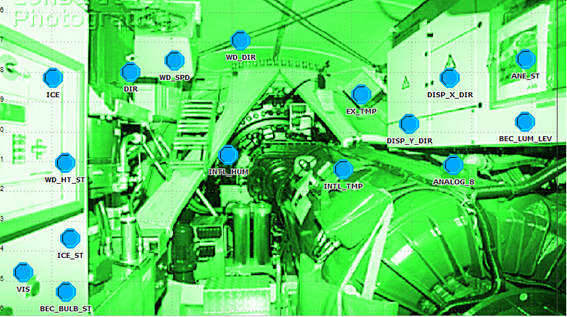
\includegraphics[width=\columnwidth]{Resim/Sekil4-2.png}}
\caption{Tübin içi \gls{wnac} modülünün temsili gösterimi. Resim kaynağı (\protect\citeA{ltd_2005}).}
\label{fig:4-2}
\end{figure}


\begin{figure}[htbp]
\centerline{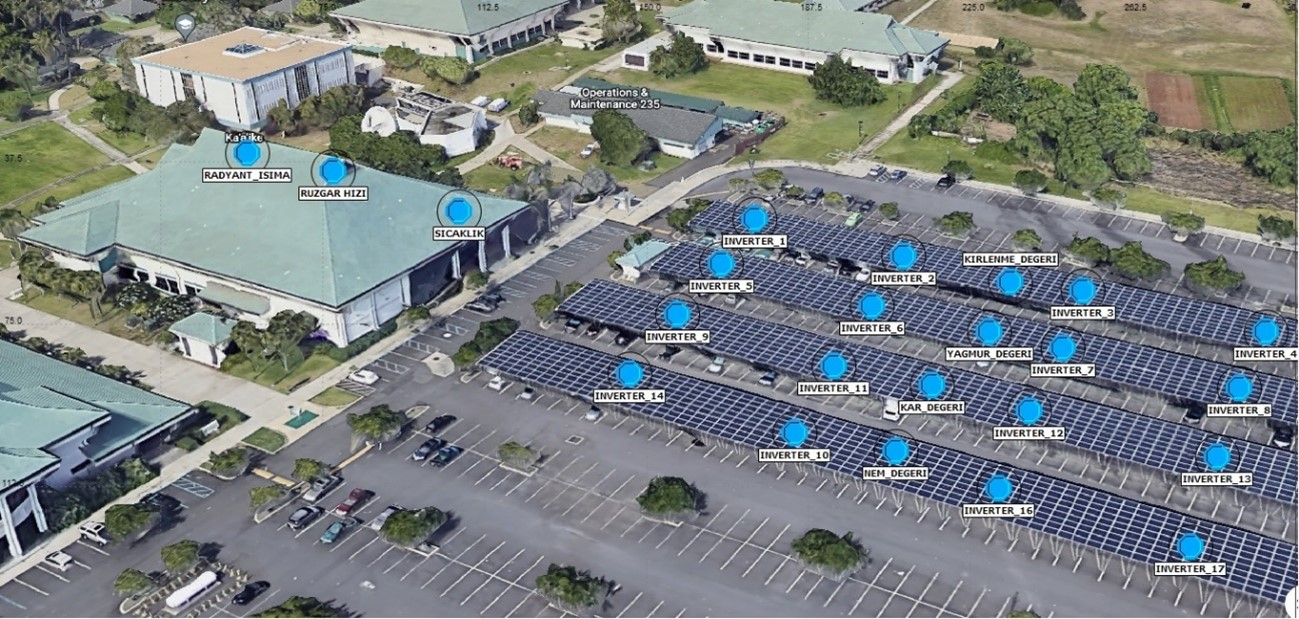
\includegraphics[width=\columnwidth]{Resim/sekil4-3.jpg}}
\caption{OPNET yazılımında güneş enerki sisteminde çalışan algılayıcı modüllerin gösterimi, enerji sisteminin resim kaynağı (\protect\citeA{inc_2015}).}
\label{fig:4-3}
\end{figure}


\subsection{Algılayıcı Düğümlerin Veri Boyutu Hesaplanması}\label{verboyut}

Bu bölüm, rüzgar türbini ve güneş enerji tarlalarında durum izleme ve arıza tahmini görevlerini gerçekleştirmek için çalışan algılayıcı düğümlerinin oluşturduğu veri boyutlarını açıklamaktadır. İlgili algılayıcıların temel prensipleri 4.1.1 ve 4.1.2 başlıkla-rında açıklanmıştır.


Yenilenebilir enerji sistemlerinde çalışan algılayıcı düğümlerinin oluşturdukları veri boyutu Denklem \eqref{eq4-1}'de hesaplanır\cite{ahmed2011simulation}.


Denklem \eqref{eq4-1}'de hesaplanır. 

\begin{equation}
\text{Veri hızı} = 2.\text{f\textsubscript{s}} \label{eq4-1}
\end{equation}

Mantıksal düğümlerden çıkan veriler örneklendiğinde 2 Byte’lık veri üretilecek şekilde tasarlanmıştır. Örnekleme frekansıyla çarpıldığı zaman mantıksal düğümün bir saniyede oluşturduğu veri boyutu hesaplanmış olur.

Mantıksal düğümler, ilgili bileşenle ilgili farklı türde bilgileri tutabilen bir veri sahibidir. Gerçek cihazla ilgili sanal model tarafından modellenen iyi bilinen fonksiyonlardır ve işlevselliğine dayalı bir veri listesi içerirler. Ek olarak mantıksal düğümlerde oluşan verilerin doğruluğu çok önemli olduğundan TCP/IP tekniği ile veri iletimi ve FTP uygulama katmanı ile çalışan bir haberleşme temelinde tasarlanmıştır. \cite{klise2017application} makalede tasarlanan veri modeli üzerinden gidildiğinde rüzgar enerji sistemi ve güneş enerji sisteminde çalışan algılayıcıların oluşturduğu veri boyutları Tablo \ref{tab:tablo4-4} ve Tablo \ref{tab:tablo4-5}’te gösterilmiştir.

\begin{table}[htbp]
\centering
\caption{Rüzgar türbinindeki algılayıcı gruplarının ürettiği veri boyutları}
\label{tab:tablo4-4}
\begin{tabular}{cccc}
\multicolumn{1}{c}{\begin{tabular}[c]{@{}c@{}}Algılayıcı modül\\ isimleri\end{tabular}} &
  \begin{tabular}[c]{@{}c@{}}Durum algılayıcı\\ veri boyutu (f\textsubscript{s} = 1)\end{tabular} &
  \begin{tabular}[c]{@{}c@{}}Analog algılayıcı\\ veri boyutu (f\textsubscript{s} = 500)\end{tabular} &
  \begin{tabular}[c]{@{}c@{}}Toplam aktarılan\\ veri\end{tabular} \\ \hline
WROT & 5*2*f\textsubscript{s} = 10 Byte/s & 5*2*f\textsubscript{s} = 10 Byte/s     & 12010 Byte/s \\
WTRM & 8*2*f\textsubscript{s} = 16 Byte/s & 12*2*f\textsubscript{s} = 1200 Byte/s  & 12016 Byte/s \\
WGEN & 2*2*f\textsubscript{s} = 4 Byte/s  & 14*2*f\textsubscript{s} = 14000 Byte/s & 14004 Byte/s \\
WCNV & 2*2*f\textsubscript{s} = 4 Byte/s  & 15*2*f\textsubscript{s} = 15000 Byte/s & 15004 Byte/s \\
WTRF & 3*2*f\textsubscript{s} = 6 Byte/s  & 8*2*f\textsubscript{s} = 8000 Byte/s   & 8006 Byte/s  \\
\gls{wnac} & 4*2*f\textsubscript{s} = 8 Byte/s  & 11*2*f\textsubscript{s} = 11000 Byte/s & 11008 Byte/s \\
WYAW & 2*2*f\textsubscript{s} = 4 Byte/s  & 6*2*f\textsubscript{s} = 6000 Byte/s   & 6004 Byte/s  \\
WTOW & 3*2*f\textsubscript{s} = 6 Byte/s  & 2*2*f\textsubscript{s} = 2000 Byte/s   & 2006 Byte/s  \\
WMET & 0                  & 8*2*f\textsubscript{s}= 8000 Byte/s    & 8000 Byte/s 
\end{tabular}
\end{table}

İlgili tablolara göre OPNET yazılımında oluşturulan rüzgar türbinindeki sensör düğümlerinin yapısı için OPNET yazılımında “Application config” eklenerek \gls{iec} 61400-25 ve \gls{iec} 61724 standartlarına göre ANALOG ve STATUS verileri aşağıdaki şekildeki gibi oluşturulur.

\begin{table}[htbp]
\centering
\caption{Güneş enerji tarlasındaki algılayıcı gruplarının ürettiği veri boyutları}
\label{tab:tablo4-5}
\begin{tabular}{lc}
\multicolumn{1}{c}{\begin{tabular}[c]{@{}c@{}}Algılayıcı modül isimleri\end{tabular}} & A sınıfı (yüksek tutarlılık periyodu) \\ \hline
Radyant ışıma              & 1*2*100 = 200 Byte/s    \\
Meteorolojik               & 5*2*1 = 10 Byte/s       \\
Rüzgar hızı                & 1*2*3 = 6 Byte/s        \\
İnverter (Gerilim ve Akım) & 2*2*1440 = 28800 Byte/s
\end{tabular}
\end{table}

OPNET yazılımında “Application Definition” modülü eklenir. İlgili modüle sağ tıklanarak “Attribute” kısmından enerji sistemlerinde çalışacak algılayıcı düğümlerinin verilerinin yapıları Şekil \ref{fig:4-4}’teki gibi tasarlanır. “Application Definition” modülünde tasarlanan uygulama verilerinin, ağ senaryolarında kullanılması için “Profil Definition” modülüne entegre edilmesi gerekir. 


\begin{figure}[htbp]
\centerline{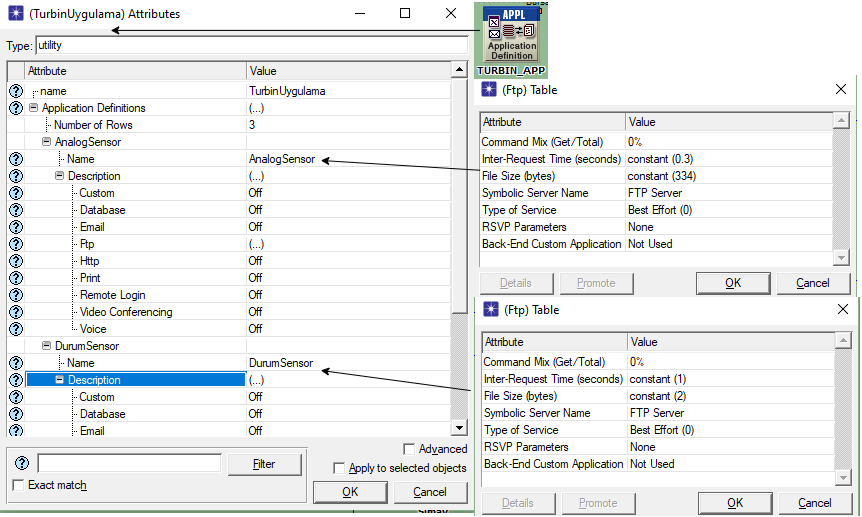
\includegraphics[width=\columnwidth]{Resim/sekil4-4.png}}
\caption{OPNET Yazılımında “Application Config” bölümü}
\label{fig:4-4}
\end{figure}

Örneğin, invertör profiline ait güneş panelinde voltaj ve akım algılayıcısı olarak iki adet algılayıcı modeli bulunmaktadır. Bu kritere göre OPNET yazılımının “Application Config” modülünde Voltaj ve Akım algılayıcılarının veri yapıları oluşturulur. İkinci aşamada ise oluşturulan bu veri yapıları “Profil Definition” modülü kullanılarak invertör profili çatısında toplanır. Böylelikle invertör profili OPNET’in ağ senaryolarında kullanımı sağlanmış olur.

Örneğin, invertör profiline ait güneş panelinde voltaj ve akım algılayıcısı olarak iki adet algılayıcı modeli bulunmaktadır. Bu kritere göre OPNET yazılımının “Application Config” modülünde Voltaj ve Akım algılayıcılarının veri yapıları oluşturulur. İkinci aşamada ise oluşturulan bu veri yapıları “Profil Definition” modülü kullanılarak invertör profili çatısında toplanır. Böylelikle invertör profili OPNET’in ağ senaryolarında kullanımı sağlanmış olur.

\begin{figure}[htbp]
\centerline{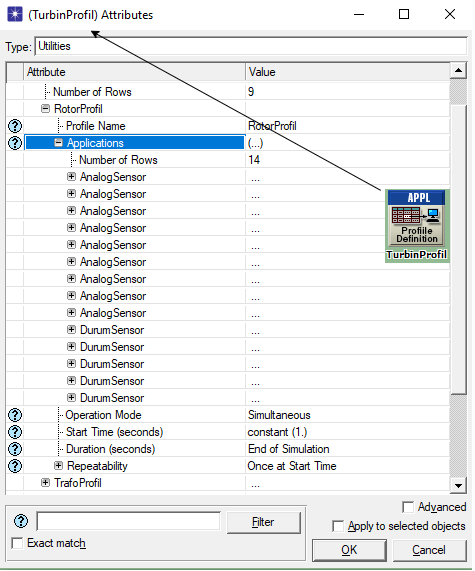
\includegraphics[width=8cm]{Resim/sekil4-5.png}}
\caption{OPNET Yazılımında “Profile Definition bölümü}
\label{fig:4-5}
\end{figure}


OPNET yazılımındaki profil config bileşeni kullanılarak yukarıdaki gibi sensör düğüm profili oluşturulur. Şekil \ref{fig:4-5}’te \gls{wnac} profilinin yapısı görülmektedir. Tablo \ref{tab:tablo4-4}’e göre \gls{wnac}'a ait olan 11 adet analog algılayıcı ve 4 adet durum (status) algılayıcısının bütün halde çalıştırıldığı profil kurulmuştur. Rüzgar türbininde enerji üretimi gerçekleşir-ken eş zamanlı çalışan \gls{wnac} gibi toplamda 9 adet algılayıcı düğüm modül grubu ve güneş enerji sisteminde kullanılan 9 adet algılayıcı düğüm modül grubu, OPNET yazı-lımındaki “Application config” ve “Profile config” bileşenleri kullanı-larak simülasyon ortamında çalışan algılayıcı gruplarına dönüştürülmüştür.



\subsection{OPNET Yerel Ağ Tasarım ve Simülasyon Sonuçları}

\begin{figure}[htbp]
\centerline{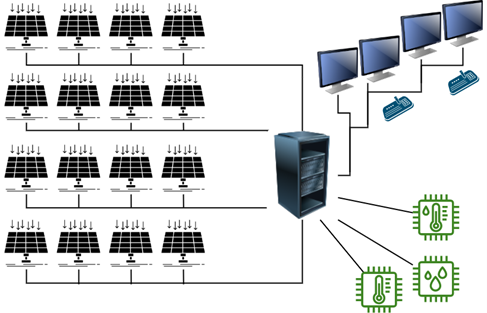
\includegraphics[width=8cm]{Resim/Sekil4-6.png}}
\caption{Güneş enerji sistemi haberleşme topolojisi}
\label{fig:4-6}
\end{figure}

Şekil \ref{fig:4-6}’da sahada kurulu olarak çalışan güneş enerji panelleri ve hava durumu algılayıcılarının sistem odasında bulunan sunucuyla bağlantısı ve sunucu ile komuta kontrol merkezinde bulunan görüntüleme bilgisayarları arasındaki bağlantının topolojisi gösterilmiştir. İlgili topoloji sadece yerel ağı gösteren bir topoloji olduğu unutulmamalıdır. Geniş ağ tasarımı hakkında yapılan çalışmalar, ayrı bir başlıkta incelenmiştir.

\subsubsection{Ethernet Teknolojisi Yerel Ağ Tasarımı}\label{yerelEthernet}


\paragraph{Güneş Enerji Sistemi}

\begin{figure}[htbp]
\centerline{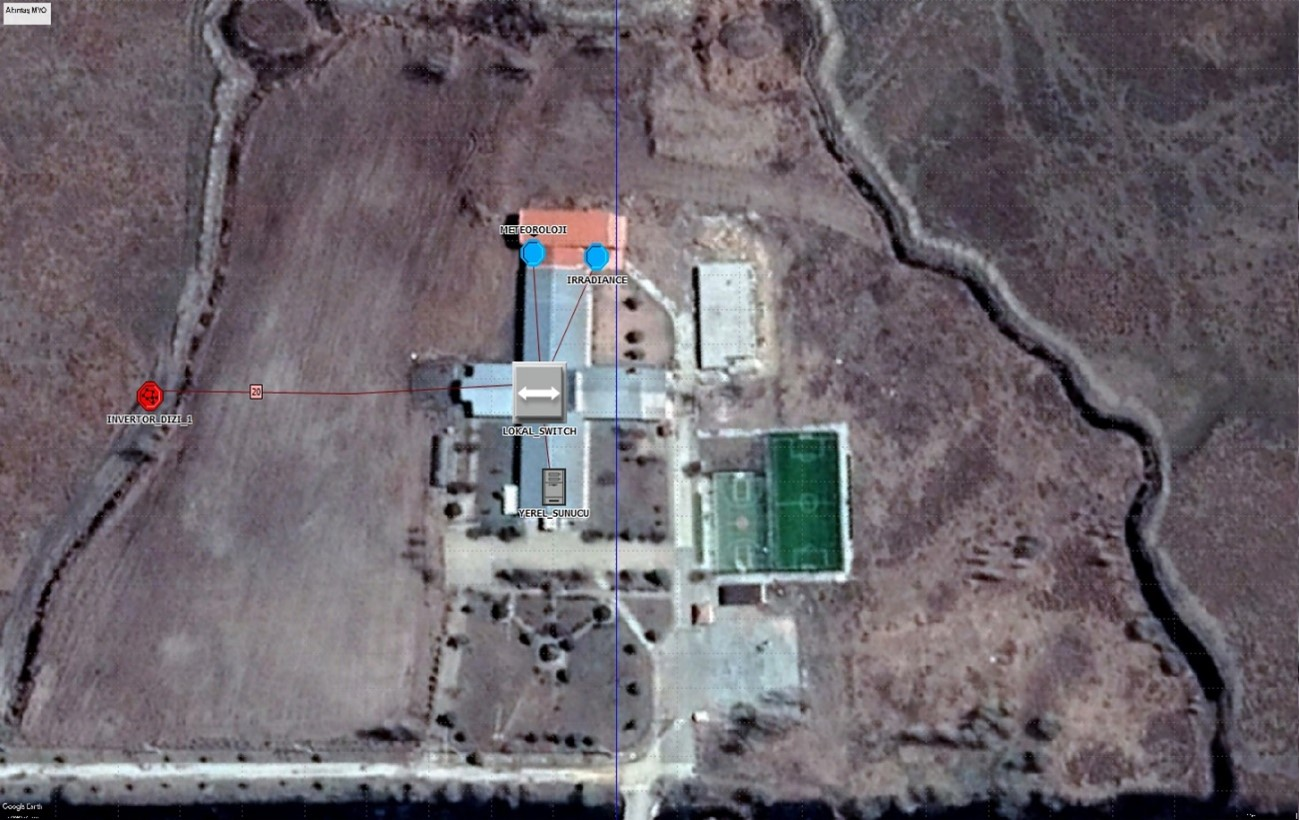
\includegraphics[width=8cm]{Resim/Sekil4-7.jpg}}
\caption{Altıntaş \gls{myo}'nun ethernet altyapısı kullanıldığı OPNET yazılımda tasarım modeli.}
\label{fig:4-7}
\end{figure}

Ethernet altyapısında haberleşme tekniği çalışan güneş enerji sisteminin maliyet ve performans değerleri ile Altıntaş \gls{myo}’nun OPNET ortamında simüle edilmiştir.

4.2.3 bölümündeki ilgili tabloda güneş enerji sisteminde kullanılan algılayıcı modüllerine göre OPNET yazılımında oluşturulan ağ yapısının görseli Şekil \ref{fig:figure9}'dedir. İlgili ağ yapısının tasarımı için OPNET yazılımında seçilmiş Ethernet sensör düğümünün detayı şekil \ref{fig:4-9}’da gösterilmiştir. 3.2.1.5 bölümünde tanımlanan Ethernet algılayıcısının şemasındaki ile uyumlu bir tasarım OPNET yazılımında modeli bulunmaktadır.

Yerel enerji üretim durumunu kontrol edebilmek için komuta kontrol merkezi ile enerji üretim sisteminin haberleşme gecikmesinin 1 saniyenin altında olması ve paket trafiğinin minimum gecikmeyle komuta merkezine aktarılması gerektiği \gls{iec} 61724 standardının temel kriteridir. Bu kritere göre tasarlanan topolojide gözlemlenen performans değerleri Şekil \ref{fig:4-10}--\ref{fig:4-12}’lerde paylaşılmıştır.


\begin{figure}[htbp]
\centerline{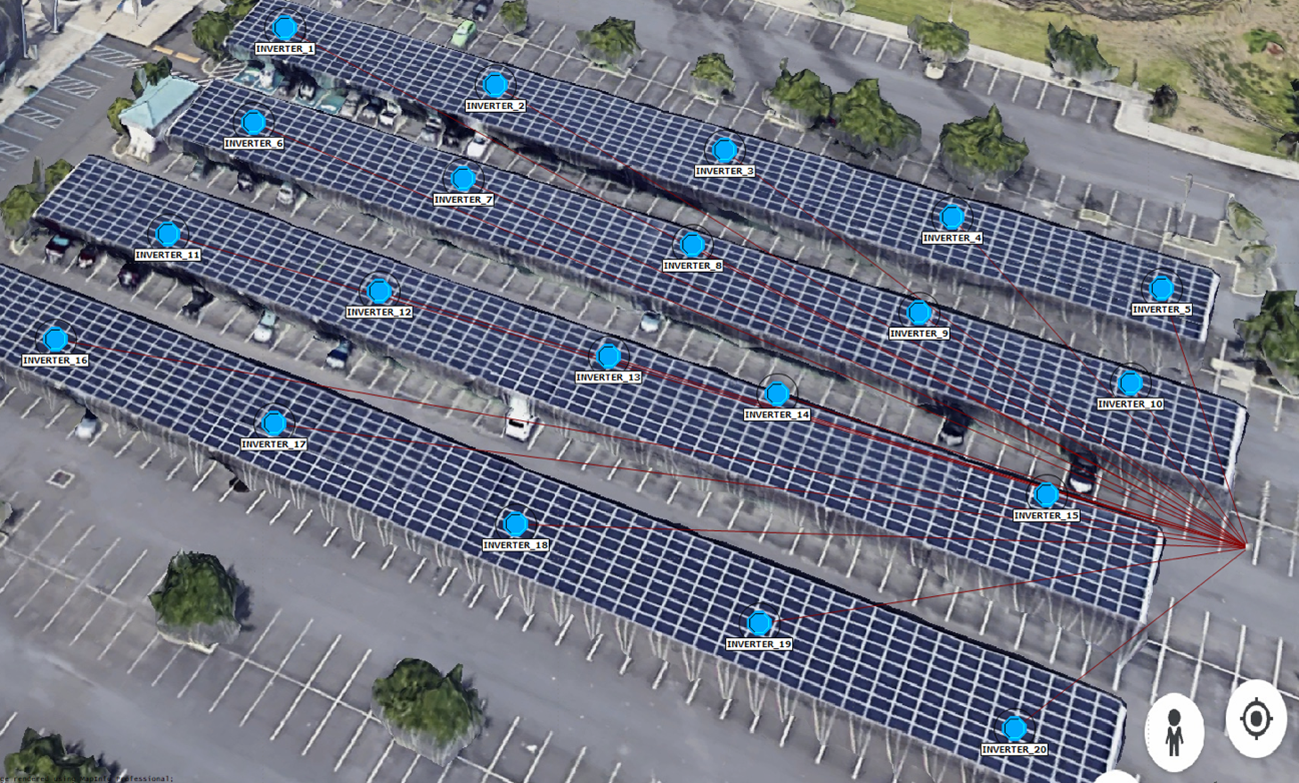
\includegraphics[width=10cm]{Resim/Sekil 4-8.png}}
\caption{Kampüs ortamında kurulan örnek güneş enerji santralinin invertör dizi grubunun OPNET yazılımında tasarlanması.}
\label{fig:4-8}
\end{figure}

\begin{figure}[htbp]


\centerline{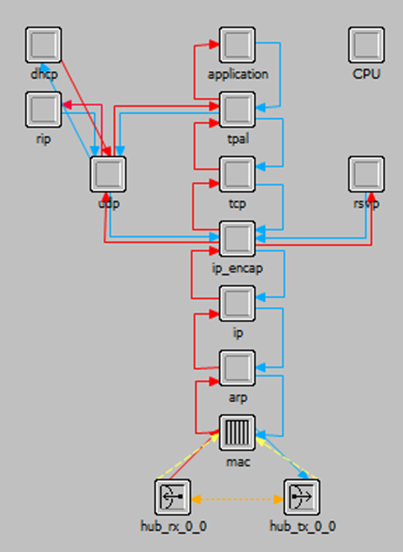
\includegraphics[width=4cm]{Resim/Sekil4-9.png}}
\caption{OPNET yazılımda tasarlanan ethernet tipi sensörlerin görüntüsü.}
\label{fig:4-9}
\end{figure}

\begin{figure}[htbp]
\centerline{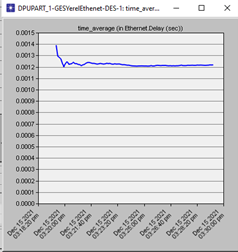
\includegraphics[width=5cm]{Resim/sekil4-10.png}}
\caption{\gls{lan}'da ethernet haberleşmesinde gözlenen gecikme değeri}
\label{fig:4-10}
\end{figure}

\begin{figure}[htbp]
\centerline{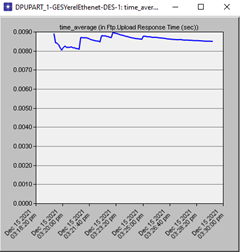
\includegraphics[width=5cm]{Resim/sekil4-11.png}}
\caption{\gls{lan}'da algılayıcılardan gönderilen verilerin yerel sunucuya yüklenme süresi}
\label{fig:4-11}
\end{figure}

\begin{figure}[htbp]
\centerline{\includegraphics[width=5cm]{Resim/şekil4-12.png}}
\caption{\gls{lan}'da 1 adet \gls{myo}'ya ait yerel sunucuya yüklenen veri grubunun logaritmik değeri}
\label{fig:4-12}
\end{figure}




\newpage


\paragraph{Rüzgar Enerji Sistemi}

Ethernet haberleşmesinde \gls{utp} kablolamanın en büyük sıkıntısı mesafedir. Veri aktarımında 100 metrede 24,6dB güç kaybı olmasından dolayı mutlaka cihaz aralarına güçlendirici kullanılması gerekmektedir. \cite{yilmazanalysis} Tezde model olarak kullanılan rüzgar türbinlerinin yüksekliği 80 metre civarındadır \cite{bauer_2010}. Algılayıcı düğüm modüllerinden gelen Ethernet kabloları türbinin zemininde bulunan bir toplayıcı anahtara gelmektedir. Toplayıcı anahtar ile lokal sunucunun olduğu komuta merkezindeki yönetim anahtarına \gls{utp} kablo bağlantısı vardır. Farklı kablo altyapıları kullanılarak haberleşme sağlanabilir örnek olarak fiber optik kablosu seçildiğinde optik kablo için Ethernet anahtarı arasına konulacak bir fiber dönüştürücü modül ve fiber kablolarının “arc fusion” tekniği ile sonlandırması kutusu ve yan ekipmanlarına ihtiyaç duyulacaktır. Bu tasarımın getireceği ekstra malzemeler bir maliyet unsuru oluşturacağından sadece \gls{utp} kablolama ile çözüme gidilme tercihi edildiği kabul edilmiştir.

\begin{figure}[htbp]
\centerline{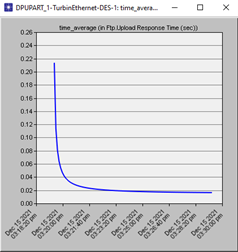
\includegraphics[width=6cm]{Resim/sekil4-13.png}}
\caption{Algılayıcılardan gönderilen verilerin yerel sunucuya yüklenme süresi}
\label{fig:4-13}
\end{figure}


\begin{figure}[htbp]
\centerline{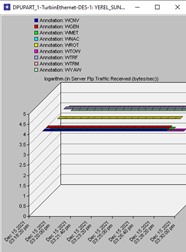
\includegraphics[width=5cm]{Resim/sekil4-14.png}}
\caption{Yerel sunucuya yüklenen veri grubunun logaritmik değeri}
\label{fig:4-14}
\end{figure}

\begin{figure}[htbp]
\centerline{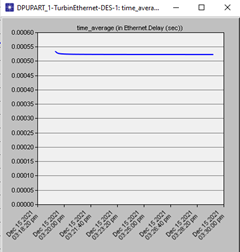
\includegraphics[width=5cm]{Resim/sekil4-15.png}}
\caption{Ethernet haberleşmesinde yaşanan gecikme}
\label{fig:4-15}
\end{figure}

Yerel enerji üretim durumunu kontrol edebilmek için komuta kontrol merkezi ile enerji üretim sisteminin haberleşme gecikmesinin 1 saniyenin altında olması ve paket trafiğinin minimum gecikmeyle komuta merkezine aktarılması gerektiği \gls{iec} 61400-25 standardının temel kriteridir. Bu kritere göre tasarlanan topolojinin performans değerleri Şekil \ref{fig:4-13}--\ref{fig:4-15}’de paylaşılmıştır.

\subsubsection{\gls{wifi} Teknolojisi Yerel Ağ Tasarımı}\label{yerelWifi}

\paragraph{Güneş Enerji Sistemi}

\gls{wifi} altyapısında haberleşme tekniği çalışan güneş enerji sisteminin maliyeti ve performans değerleri ile Altıntaş \gls{myo}’nun OPNET ortamında simülasyonunun raporları bu bölümde paylaşılmıştır.


\begin{figure}[htbp]
\centerline{\includegraphics[width=5cm]{Resim/Ekran görüntüsü 2022-05-01 220615.jpg}}
\caption{OPNET yazılımındaki \gls{wifi} algılayıcı düğümü}
\label{fig:4-16}
\end{figure}


Yerel enerji üretim durumunu kontrol edebilmek için komuta kontrol merkezi ile enerji üretim sisteminin haberleşme gecikmesinin 1 saniyenin altında olması ve paket trafiğinin minimum gecikmeyle komuta merkezine aktarılması gerektiği \gls{iec} 61724 standardının temel kriteridir. Bu kritere göre tasarlanan topolojinin performans değerleri Şekil \ref{fig:4-17}--\ref{fig:4-19}’da paylaşılmıştır

\begin{figure}[htbp]
\centerline{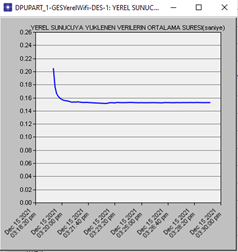
\includegraphics[width=5cm]{Resim/sekil4-16.png}}
\caption{Yerel sunucuya yüklenen verilerin ortalama süresi}
\label{fig:4-17}
\end{figure}


\begin{figure}[htbp]
\centerline{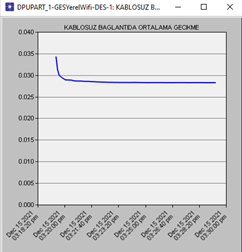
\includegraphics[width=5cm]{Resim/sekil4-17.png}}
\caption{Yerel ağda yaşanan gecikme süresi}
\label{fig:4-18}
\end{figure}

İlgili simülasyon sonuçlarına göre güneş enerji santralinin haberleşme standartlarında bir ihlal durumu olmadan sağlıklı bir şekilde yerel sunucuya verilerin aktarıldığı gözlemlenmiştir.

\begin{figure}[htbp]
\centerline{\includegraphics[width=5cm]{Resim/Sekil4-18.png}}
\caption{Yerel sunucuya yüklenen veri gruplarının logaritmik değeri}
\label{fig:4-19}
\end{figure}

\paragraph{Rüzgar Enerji Sistemi}

Domaniç \gls{myo}'nun rüzgar enerji sistemindeki haberleşme altyapısı \gls{wifi} olarak OPNET ortamında kurulduktan sonra gözlenen simülasyon sonuçları Şekil \ref{fig:4-20}-\ref{fig:4-22}’de paylaşılmıştır.

\begin{figure}[htbp]
\centerline{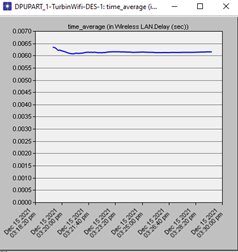
\includegraphics[width=5cm]{Resim/Sekil4-19.png}}
\caption{Yerel ağda yaşanan gecikme süresi}
\label{fig:4-20}
\end{figure}

\begin{figure}[htbp]
\centerline{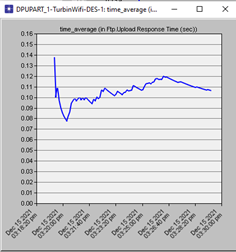
\includegraphics[width=5cm]{Resim/Sekil4-20.png}}
\caption{Yerel sunucuya yüklenen verilerin ortalama süresi}
\label{fig:4-21}
\end{figure}


\begin{figure}[htbp]
\centerline{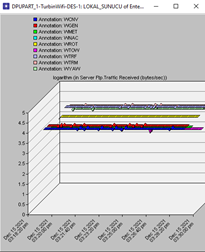
\includegraphics[width=5cm]{Resim/Sekil4-21.png}}
\caption{Yerel sunucuya yüklenen veri gruplarının logaritmik değeri}
\label{fig:4-22}
\end{figure}

\newpage
\subsubsection{Zigbee Teknolojisi Yerel Ağ Tasarımı}\label{zigbee}


Zigbee haberleşme altyapısı \gls{wifi} ve ethernet haberleşme teknolojilerine göre çok daha ucuzdur fakat, \gls{iec}'nin belirlemiş olduğu gerçek zamanlı izleme standartlarına uymadığı gözlemlenmiştir. Önceki kısımlardaki gibi aynı noktalarda kurulan enerji sistemlerinin algılayıcı verilerinin oluşturmuş olduğu veri trafiğinin performans değerleri aşağıdaki başlıklarda gösterilmiştir.


\paragraph{Güneş Enerji Sistemi}

\begin{figure}[htbp]
\centerline{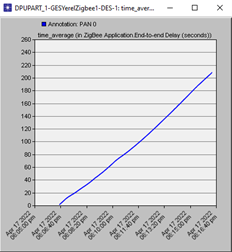
\includegraphics[width=5cm]{Resim/Sekil4-22.png}}
\caption{Yerel ağda yaşanan gecikme süresi}
\label{fig:4-23}
\end{figure}

\begin{figure}[htbp]
\centerline{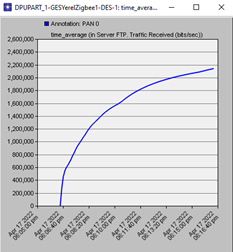
\includegraphics[width=5cm]{Resim/Sekil4-23.png}}
\caption{Yerel ağdaki sunucuda toplanan veri boyutu}
\label{fig:4-24}
\end{figure}


\paragraph{Rüzgar Enerji Sistemi}

OPNET ortamında simülasyonu yapılan rüzgar enerji sisteminin grafikleri Şekil \ref{fig:4-25} ve \ref{fig:4-26} da paylaşılmıştır.

\begin{figure}[htbp]
\centerline{\includegraphics[width=5cm]{Resim/sekil4-24.png}}
\caption{Yerel ağda yaşanan gecikme süresi}\label{fig:4-25}
\end{figure}

\begin{figure}[htbp]
\centerline{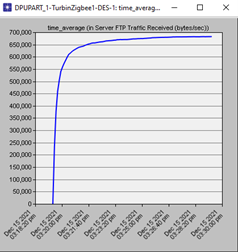
\includegraphics[width=5cm]{Resim/sekil4-25.png}}
\caption{Yerel ağdaki sunucuda toplanan veri boyutu}
\label{fig:4-26}
\end{figure}



\subsubsection{Yerel Ağ Tasarım Sonuçları}


Zigbee, \gls{wifi} ve Ethernet altyapısında modellenen simülasyonların 2 \gls{myo}'daki sonuçları \ref{yerelEthernet}--\ref{zigbee} başlıklarında paylaşılmıştır. Ağ Tasarımda paylaşılan grafikler incelendiğinde Zigbee altyapısı ile kurulan haberleşme trafiğinde gecikme değerleri ilgili standartların belirlemiş olduğu üst değer olan 1 saniyenin çok üzerindedir. Bu sebeple Geniş Ağ tasarımının olduğu bölümde yerel ağ teknolojisi varyantlarına Zigbee altyapısı dahil edilmemiştir.

\subsection{OPNET Geniş Ağ Tasarım ve Simülasyon Sonuçları}

Önceki bölümde yerel ağ tasarımı modeli incelenmiştir. Şekil \ref{fig:4-27}’de Google Earth yazılımında Kütahya’nın meslek yüksekokulları ve merkez kampüsü gösterilmiştir. Okullardaki enerji üretim sisteminin merkezi bir noktadan kontrolü gözlemi ve aksiyonu için \gls{iec}, veri haberleşmesinin en fazla 1 saniye gecikmesine izin vermiştir. Tasarım olarak enerji üretiminin izlendiği \gls{dpu} Merkez Kampüsü olarak belirlenmiştir. Geniş ağ tasarım senaryoları kablosuz ve kablolu olarak iki kısımda incelenmiştir.


\begin{figure}[htbp]
\centerline{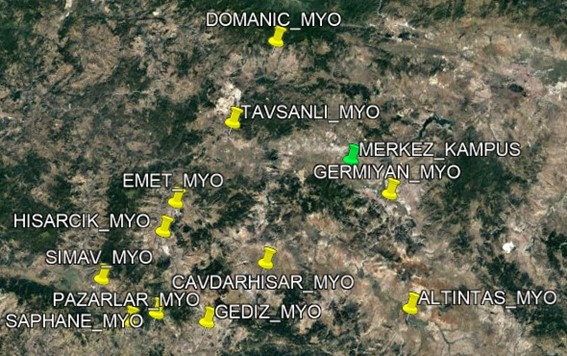
\includegraphics[width=5cm]{Resim/sekil4-26.jpg}}
\caption{\gls{dpu}’nün Meslek Yüksek Okulları ve Merkez Kampüsü}
\label{fig:4-27}
\end{figure}


\subsubsection{Kablosuz Geniş Ağ Tasarımı}

\ref{mikrohaberlesme} kısmında belirtilen mikrodalga haberleşme tekniğinden \gls{wimax} teknolojisi kullanılarak meslek yüksekokulları arasında bir haberleşme linki kurulmuştur. Yüksek hızlarda ve gerçek zamanlı haberleşme çözümü imkanı sağlayan \gls{wimax} teknolojisini 11-66 GHz arasında bir haberleşme frekansına sahiptir. Bu frekans aralığındaki elektromanyetik dalga boyunun çok küçüktür. Dalga boyunun küçük olmasından kaynaklı olarak kilometre seviyelerinde yüksek veri aktarım teknolojisini minimum kayıp ve maksimum verimle yapabilmesi için noktalar arası doğrudan görüş hattı olması gerekmektedir.

İlgi \gls{myo}'ların \gls{dpu} merkez kampüsü ile sağlıklı bir haberleşme sağlaması için öncelikle sistemsel olarak Google Earth yazılımında Kütahya ilinin fiziki yükselti haritası incelenmiştir. Bu incelemelerin sonucunda 2 adet toplama noktası belirlenmiştir. Bu toplama noktaları ile üniversiteye ait kampüsler birbirlerini doğrudan ve engelsiz bir şekilde gördüğü Google Earth yazılımından doğrulanmıştır.

Toplama noktalarıyla doğrudan haberleşen meslek yüksekokulları Tablo \ref{tab:tablo4-6}'da gösterilmiştir.



\begin{figure}[htbp]
\centerline{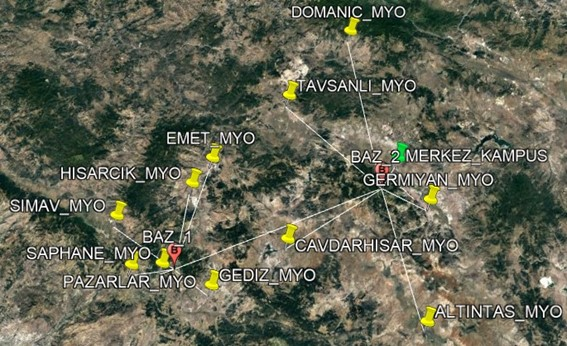
\includegraphics[width=10cm]{Resim/sekil4-27.jpg}}
\caption{Baz istasyonu vaziyet planı}
\label{fig:4-28}
\end{figure}




\begin{table}[htbp]
\centering
\caption{Yerleşkelerde kullanılan enerji sistemi ve bağlı olduğu baz istasyonları.}
\label{tab:tablo4-6}
\begin{tabular}{|l|c|l|c|}
\hline
Yerleşke İsmi        & \multicolumn{1}{l|}{Baz No} & Yerleşke İsmi         & \multicolumn{1}{l|}{Baz No} \\ \hline
Pazarlar \gls{myo} (Güneş) & \multirow{6}{*}{1}          & Tavşanlı \gls{myo} (Rüzgar) & \multirow{6}{*}{2}          \\ \cline{1-1} \cline{3-3}
Hisarcık \gls{myo} (Rüzgar) &  & Domanic \gls{myo} (Rüzgar)    &  \\ \cline{1-1} \cline{3-3}
Şaphane \gls{myo} (Güneş)   &  & Germiyan \gls{myo} (Rüzgar)   &  \\ \cline{1-1} \cline{3-3}
Gediz \gls{myo} (Güneş)     &  & Altıntaş \gls{myo} (Güneş)    &  \\ \cline{1-1} \cline{3-3}
Simav \gls{myo} (Rüzgar)    &  & Çavdarhisar \gls{myo} (Güneş) &  \\ \cline{1-1} \cline{3-3}
Emet \gls{myo} (Rüzgar)     &  & Merkez Kampüs (İzleme)  &  \\ \hline
\end{tabular}
\end{table}


\begin{figure}[htbp]
\centerline{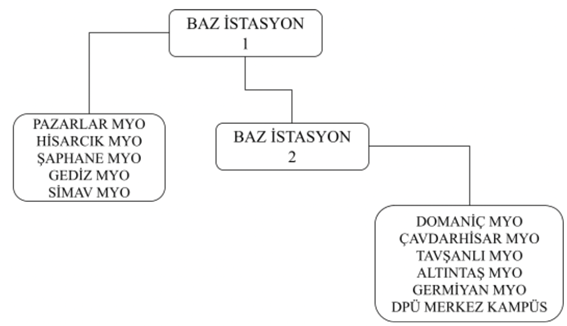
\includegraphics[width=10cm]{Resim/sekil4-28.png}}
\caption{Baz istasyonları bağlantı topolojisi}
\label{fig:4-29}
\end{figure}

\gls{wimax} haberleşmesinde bant genişliği çok önemli bir faktördür. Gereksiz bant tutan veri trafiği en istenmeyen durumdur. Tezin amacında da belirtildiği üzere amaçlanan kriter minimum haberleşme maliyeti ile maksimum verimli bir haberleşme çözümü sunmaktır. Bu nedenle lokal bölgelerde oluşturulan verilerin \gls{dpu} Merkez kampüsüne ileti-lirken diğer lokal bölgelere iletilmesinin önüne geçilmelidir. 

Günümüzde IP haberleşmesinde farklı ağları birbirleriyle haberleştirme tekniği olarak yönlendirme protokolleri kullanılmaktadır. 
Kullanıcı kendi yerel ağ dışındaki bir noktaya veri gönderebilmesi için yerel ağındaki yönlendiriciye verisini iletir, yönlendirici nihai hedefe doğru verileri iletmektedir, nihai hedefin yerel ağ segmentinden sorumlu yönlendiriciye kadar belirli cihazlar arasında atlama yapmaktadır. Uçtan uca yol boyunca her yönlendirici, hedefe ulaşmak için kullanılan bir sonraki atlama cihazını seçer. Sonraki atlama, hedefe ulaşmak için yol boyunca bir sonraki cihazı temsil eder. Böylelikle rotalama tekniği uygulanmış olur. 

IP yönlendirme metodu statik ve dinamik olarak iki kısımda incelenir. Bu tezde veri trafiklerini geniş alan ağlarında yönetmek için statik yönlendirme kullanılmıştır.

Statik yönlendirme, ağ yöneticisi tarafından tasarlanır ve ağa uygulanır. Ağ yöneticisinin sorumluluğunda bütün trafik şekillenmektedir. Statik yönlendirmenin tercih edilme sebepleri aşağıda paylaşılmıştır. \cite{parziale_2006}

•	Yönlendirme algoritmasına göre daha spesifik bir rota içermediğinde trafiği iletmek için tercih edilir.

•	Karmaşık yönlendirme ilkeleri gerektiğinde kullanılır. Örnek olarak, belirli bir ana bilgisayara yönlendirilen trafiğin belirlenmiş bir ağ yolundan geçmesini garanti etmek gibi bir senaryo gerektiğinde statik yönlendirme tekniği kullanılır.

•	Ağ yöneticisi, kurulu sistemde tanımlanan tüm ağların sınıfı veya özelliğine göre birbirleriyle spesifik verilerin haberleşmesini sağlamak için statik yönlendirme kullanmaktadır. 

•	Statik yönlendirme yöntemi, komşu cihazlar arasında rota bilgilerini tanıtmayı gerektirmez. Bu durum sayesinde haberleşmede kullanılan bant genişliğinden tasarruf edilir. Ayrıca, ağ yollarını hesaplamak için daha az işlemci önbelleği ve döngüsü kullanır.

\gls{wimax} teknolojisinde veri trafiğinde kullanılan bant genişliği çok önemli bir konudur. Bilindiği üzere \gls{wimax} lisanslı bir bant üzerinden haberleşmesini yapmaktadır, yani limitli bir bant genişliği kullanımı söz konusudur. Bu nedenle yerel noktalarda oluşturulan verilerin en az bant kullanılarak gönderilmesi amaçlanmıştır. Statik yönlendirme tekniği de bu sebepten kullanılmaktadır. Bu teknik sayesinde aynı baz istasyonlarına bağlı farklı meslek yüksekokulları, birbirlerinin haberleşme bant genişliğini işgal etmemektedir. Merkez noktadaki toplama noktasına gönderilen veriler böylelikle korunmuş olur ayrıca başka noktalara gönderilmeden kaynaklı gereksiz bant kullanımının önüne geçilmiş olur.

\begin{figure}[htbp]
\centerline{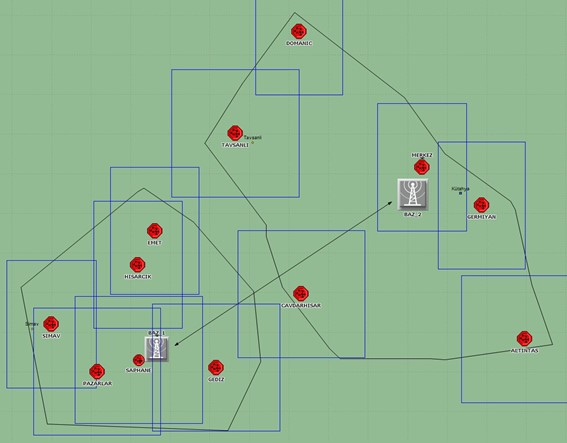
\includegraphics[width=10cm]{Resim/sekil4-29.jpg}}
\caption{OPNET yazılımında tasarlanan WAN topolojisi}
\label{fig:4-30}
\end{figure}



\paragraph{Yerel Ağ Teknolojisi = \gls{wifi} \& Geniş Ağ Teknolojisi \gls{wimax}}

Yerel ağ teknolojisindeki \gls{wifi} sistemlerinin tümündeki gözlemlenen gecikme (delay) değeri ortalama 0.06 saniye değerindedir. Şekil \ref{fig:4-31}’de gözlemlenen gecikme değeri \gls{iec} 61400 ve \gls{iec} 61724 standartlarını karşılamaktadır. 12 adet kampüs içi yerel ağın \gls{wifi} üzerinden haberleşme yapılması durumuyla birleştirilmiş \gls{wimax} geniş alan ağı teknolojisinde yaşanan gecikmenin grafiği Şekil \ref{fig:4-31}’de paylaşılmıştır.



\begin{figure}[htbp]
\centerline{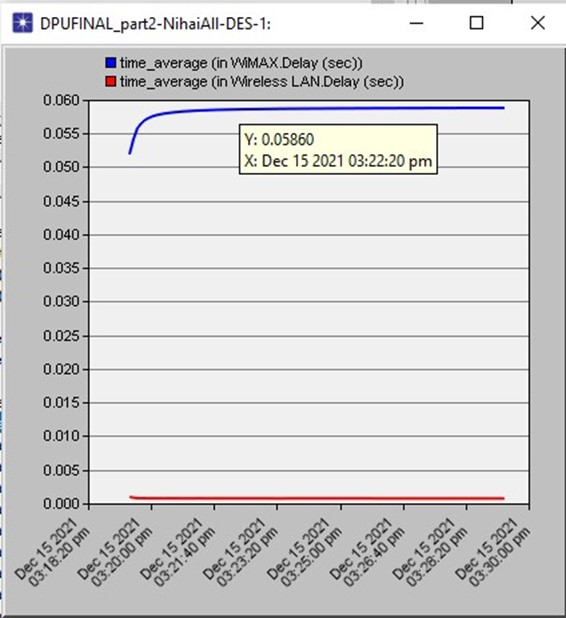
\includegraphics[width=10cm]{Resim/Sekil4-30.jpg}}
\caption{\gls{wimax} ve \gls{wifi} teknolojisinde gözlemlenen gecikme değeri}
\label{fig:4-31}
\end{figure}

\gls{dpu}'nün merkez kampüsünde kurulan ana sunucuya gönderilen toplam veri boyutunun anlık olarak grafiği Şekil \ref{fig:4-32}’de gösterilmiştir. Yerel ağlarda kurulu olan güneş ve rüzgar enerji sistemlerinde üretilen verilerin toplam boyutu, ana sunucuya gelen veri boyutuyla aynıdır. 11 adet \gls{myo}'da oluşturulan sensör verilerinde bir kayıp olmadığı Şekil \ref{fig:4-32}'den anlaşılmaktadır.

\begin{figure}[htbp]
\centerline{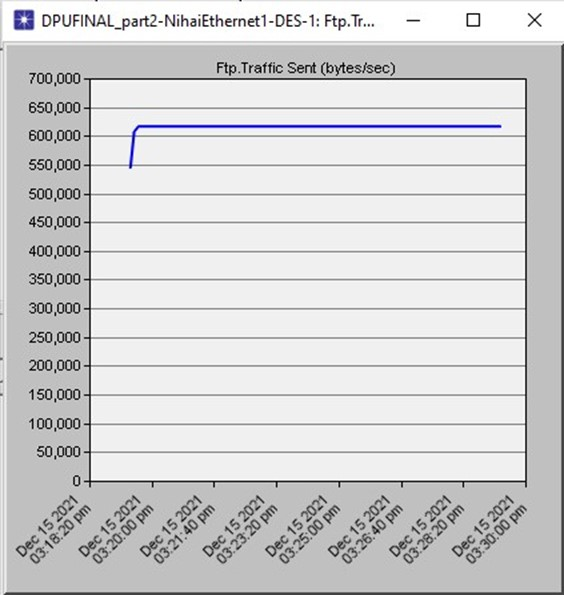
\includegraphics[width=10cm]{Resim/Sekil4-31.jpg}}
\caption{Ana sunucuda toplanan verilerin değeri}
\label{fig:4-32}
\end{figure}


Şekil \ref{fig:4-33}’te logaritmik tabanda ana sunuya gelen algılayıcı modüllerin değerleri gösterilmiştir. Grafik değerlerinin gözlemi için logaritmik tabanda sonuçlar alınmıştır. Çünkü Tablo \ref{tab:tablo4-5}’teki meteoroloji algılayıcılarının ürettikleri veri değeri 16 Byte/saniye değerinde fakat Tablo \ref{tab:tablo4-4}’teki rüzgar enerji türbininin rotor modülü 12010 Byte/saniye değerinde veri üretmektedir. İki değerin de rahatça grafikte gözlemlenebilinmesi için logaritmik taban tercih edilmiştir.

\begin{figure}[htbp]
\centerline{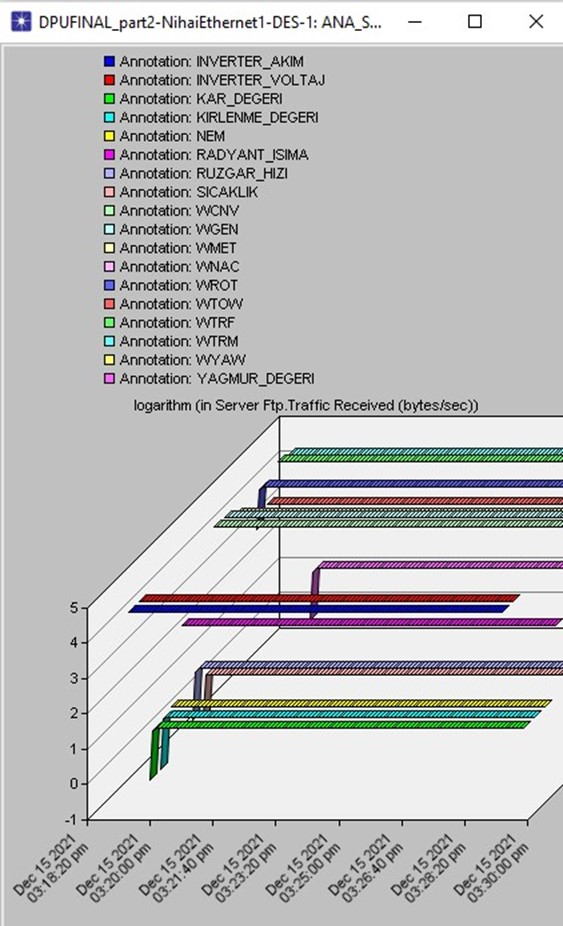
\includegraphics[width=10cm]{Resim/Sekil4-32.jpg}}
\caption{Ana sunuca toplanan algılayıcı düğümlerin logaritmik değeri}
\label{fig:4-33}
\end{figure}


Tablo \ref{tab:tablo4-6}’ya göre meslek yüksek okullarında üretilen sensör verilerinin \gls{dpu} komuta merkezi sunucusuna gönderilme zamanı Şekil \ref{fig:4-34}’de gösterilmiştir. Bu grafiğe göre üretilen veriler yaklaşık 0.46 saniyelik gecikme ile ana sunucuda toplandığı gözlem-lenmiştir. Geniş ağ teknolojisindeki \gls{iec} standartlarında verilerin 1 saniyenin altında bir süre ile hedef noktasına iletilmesi gerektiği belirtilmektedir \cite{mackiewicz2006overview}. Buna göre tasarlanan \gls{wifi} ve \gls{wimax} hibrit teknolojili haberleşme sistemi ilgili standartları tamamen karşılamaktadır

\begin{figure}[htbp]
\centerline{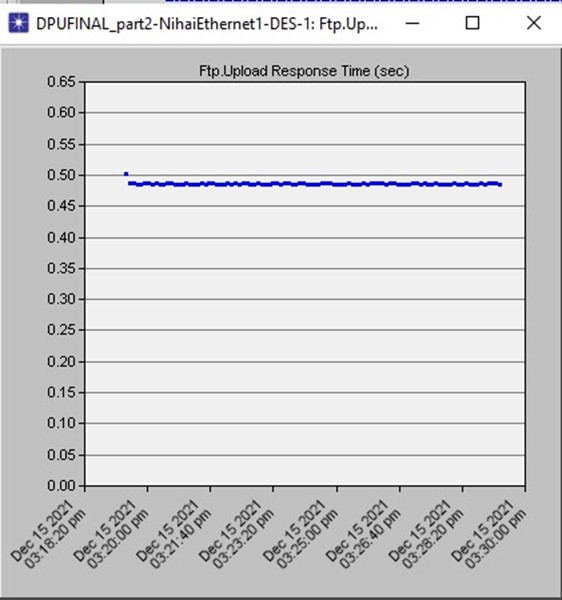
\includegraphics[width=10cm]{Resim/Sekil4-33.jpg}}
\caption{Enerji sistemlerindeki algılayıcı verilerin ana sunucuya ortalama ulaşma süresi}
\label{fig:4-34}
\end{figure}


\paragraph{Yerel Ağ Teknolojisi = Ethernet \& Geniş Ağ Teknolojisi \gls{wimax}}

Şekil \ref{fig:4-35}’te gözlemlenen yerel ağ teknolojisindeki Ethernet gecikme değeri yaklaşık 0.00015 saniyedir. \gls{wimax} gecikme değeri sistemlerinin tümündeki gözlemlenen gecikme (delay) değeri ortalama 0.06 saniye değerindedir. Bu değerler yerel ağda kullanılan \gls{wifi} teknolojisindeki değerlere göre daha iyidir.


\begin{figure}[htbp]
\centerline{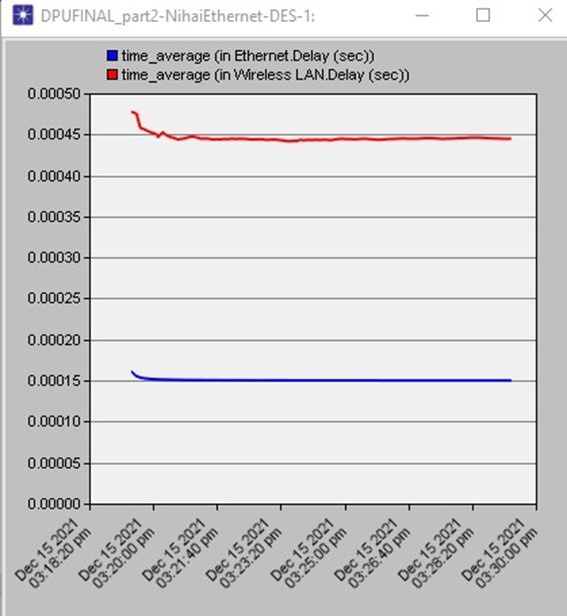
\includegraphics[width=10cm]{Resim/Sekil4-34.jpg}}
\caption{\gls{wimax} ve Ethernet teknolojisinde gözlemlenen gecikme değeri}
\label{fig:4-35}
\end{figure}

Şekil \ref{fig:4-36}’da \gls{dpu}’nün merkez kampüsünde kurulan ana sunucuya gönderilen toplam verinin grafiği gösterilmiştir. Şekil \ref{fig:4-32}’deki grafikle aynı performansı göster-miştir. Verilerin aktarım değerleri 1 saniyenin altında olduğundan, ilgili senaryodaki verimler birbirlerine çok yakın olması beklenen bir davranıştır.


\begin{figure}[htbp]
\centerline{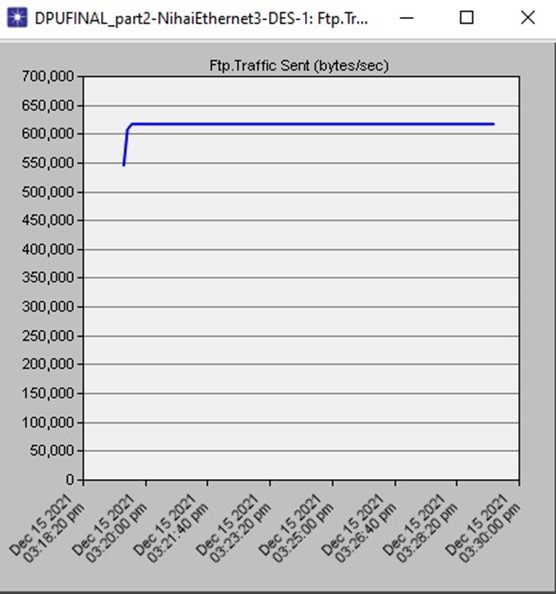
\includegraphics[width=10cm]{Resim/Sekil4-35.jpg}}
\caption{Ana sunucuda toplanan verilerin boyutu}
\label{fig:4-36}
\end{figure}


Ana sunucuda toplanan sensör modüllerin anlık değeri Şekil \ref{fig:4-37}’de görülmektedir. Yerel ağda \gls{wifi} teknolojisi kullanıldığında da aynı değerler elde edilmiştir. Buna göre haberleşme trafiğinde yerel ağ teknolojisinin Ethernet veya \gls{wifi} olması veri aktarımında bir performans değişikliği oluşturmamaktadır.

\begin{figure}[htbp]
\centerline{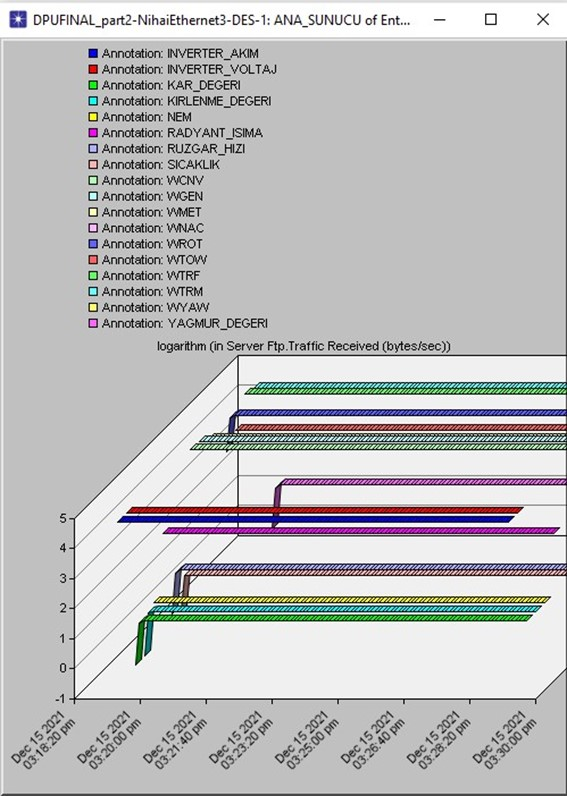
\includegraphics[width=10cm]{Resim/sekil4-36.jpg}}
\caption{Ana sunuca toplanan algılayıcı düğümlerin logaritmik değeri}
\label{fig:4-37}
\end{figure}

Tablo \ref{tab:tablo4-6}’ya göre meslek yüksek okullarında üretilen algılayıcı verilerinin \gls{dpu} \\komuta merkezi sunucusuna gönderilme zamanı Şekil \ref{fig:4-38}’de gösterilmiştir. Bu grafiğe göre üretilen veriler yaklaşık 0.41 saniyelik gecikme ile ana sunucuda toplandığı gözlemlenir. Geniş ağ teknolojisindeki \gls{iec} standartlarında verilerin 1 saniyenin altında bir süre ile hedef noktasına iletilmesi gerektiği belirtilmektedir \cite{mackiewicz2006overview}. Buna göre tasarlanan Ethernet ve \gls{wimax} hibrit teknolojili haberleşme sistemi ilgili standartları tamamen karşılamaktadır.


\begin{figure}[htbp]
\centerline{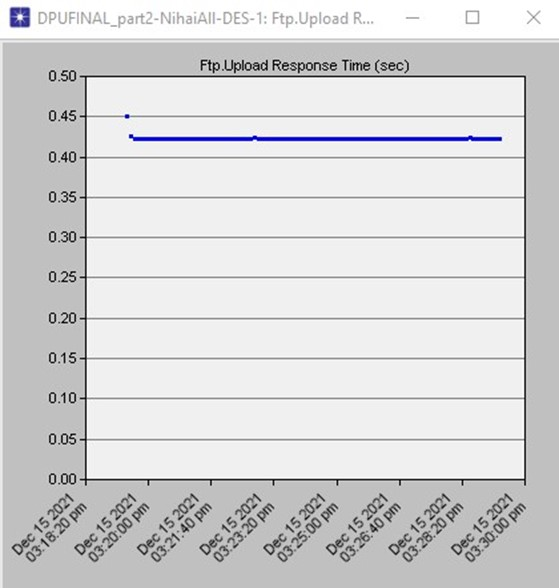
\includegraphics[width=10cm]{Resim/sekil4-37.jpg}}
\caption{Ana sunuca toplanan algılayıcı düğümlerin logaritmik değeri}
\label{fig:4-38}
\end{figure}


\subsubsection{Fiber Altyapılı Geniş Ağ Tasarımı}\label{fibeeraciklama}


Yerel internet sağlayıcıları üzerinden tarife anlaşması sağlanarak kurulmaktadır. Fakat telekom hattı sadece \gls{dpu} hizmet vermemekle birlikte hizmet sağladığı noktalardaki başka aboneleriyle birlikte ortak bir haberleşme havuzundan haberleşme hizmeti vermektedir. Bu hizmetin finansal açıdan ilk başta avantajının olması kaçınılmazdır. Fakat üniversiteye bağlı \gls{myo}'ların haberleşme güvenliğinin sağlanması son kullanıcının sorumluluğunda olacaktır. Buna göre ilgili meslek yüksekokullarına kurulacak harici bir güvenlik duvarı ve yönlendirici donanımlarıyla yerel ağlarda toplanan algılayıcı verileri fiziki bir güvenlik duvarından geçerek yönlendiriciler üzerinden \gls{dpu} Merkez kampüsüne ulaşır.


\begin{figure}[htbp]
\centerline{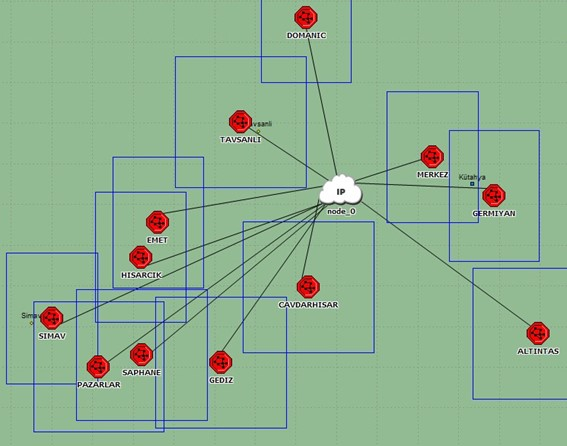
\includegraphics[width=10cm]{Resim/sekil4-39.jpg}}
\caption{Telekom altyapısındaki fiber optik hizmet tarifesinin OPNET ortamında uyarlanması}
\label{fig:4-39}
\end{figure}

Şekil \ref{fig:4-40}’da görüldüğü üzere ana sunucuya iletilen verilerin süresi paylaşılır. Verilerin fiber optik altyapıyla iletilmesi, veri hızı açısından en etkili yöntemdir.

\begin{figure}[htbp]
\centerline{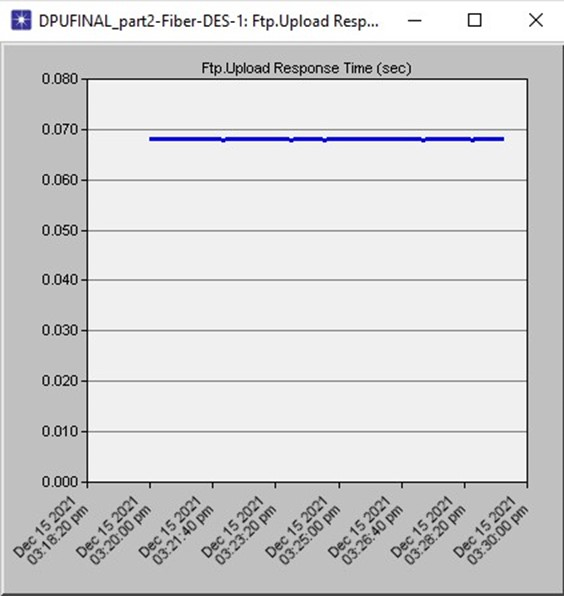
\includegraphics[width=10cm]{Resim/sekil4-38.jpg}}
\caption{Enerji sistemlerindeki algılayıcı verilerin ana sunucuya ortalama ulaşma süresi.}
\label{fig:4-40}
\end{figure}

\section{SİSTEM BİLEŞENLERİNİN MALİYET HESABI}

2022 yılı inşaat ve tesisat birim fiyat kitabına, \gls{dmo} satın alım sayfalarına, Türkiye’de Aselsan AŞ’nin yetkili \gls{wimax} bayisine ve Türk Telekom A.Ş.’nin fiyatlarına bağlı kalınarak, haberleşme sistemlerinde kurulacak malzeme ve işçi-liklerin maliyet tabloları oluşturulmuştur \cite{birimfiyat}.




\subsection{Kablolu Yerel Ağ Haberleşme Altyapısı (Güneş Enerji Sistemi)}


Kablolu haberleşme ağı altyapısında kullanılan malzemelerin işçilikli maliyeti Tablo \ref{tab:tablo4-7}’de gösterilmiştir.

İlgili tabloya bakıldığında kablolu haberleşmedeki en yüksek maliyet haberleşme sisteminin dış ortam şartlarından korunması için gereken koruyucu ekipmanlarıdır. Çünkü\\ sistemin iletiminde dış ortamdan korunması için endüstriyel ortamlarda kullanılan koruge borusu, bir arıza durumunda müdahale kolaylığı sağlanması için kullanılan menhol malzemeleri, sistemin sürdürülebilirliğini sağlaması için kritik malzemelerdir.


\begin{table}[htbp]
\centering
\caption{\gls{myo} kablolu haberleşme altyapısı maliyet tablosu}

\label{tab:tablo4-7}
\begin{tabular}{ccccr}
\hline
Malzeme tanımı &
  \begin{tabular}[c]{@{}c@{}}Bakanlık Poz\\ Numarası\end{tabular} &
  Maliyet (\Lira) &
  Miktar &
  \multicolumn{1}{c}{Toplam} \\ \hline
FTP Cat6 Kablo                                                       & 35.505.2040          & 10,00\Lira               & 1330 mt & 13.300,00\Lira           \\ \hline
PE Esaslı Menhol                                                     & 10.450.10.57         & 300,00\Lira              & 22 ad   & 6.600,00\Lira            \\ \hline
\begin{tabular}[c]{@{}c@{}}300 mm Anma\\ Çaplı HDPE\\ Koruge Boru\\ Ek Aparatları Dahil\end{tabular} &
  10.450.10.57 &
  70,00\Lira &
  700 mt &
  49.000,00\Lira \\ \hline
\begin{tabular}[c]{@{}c@{}}\gls{utp} Cat6 Patch\\ Panel\end{tabular}       & 35.505.7302          & 1.355,00\Lira            & 1 ad    & 1.355,00\Lira            \\ \hline
\begin{tabular}[c]{@{}c@{}}Dikili Tip Kabinet\\ Tüm Elemanları Dahil\end{tabular} &
  35.550.2000 &
  9.000,00\Lira &
  1 ad &
  9.000,00\Lira \\ \hline
\begin{tabular}[c]{@{}c@{}}Yönetilebilir Ağ\\ Anahtarı\end{tabular} &
  \begin{tabular}[c]{@{}c@{}}7677-K3193\\ (\gls{dmo}\\ ürün kodu)\end{tabular} &
  8.426,66\Lira &
  1 ad &
  8.426,66\Lira \\ \hline
Patch Cord                                                           & 35.545.2105          & 52,00\Lira               & 37 ad   & 1.924,00\Lira            \\ \hline
\begin{tabular}[c]{@{}c@{}}Ethernet Algılayıcı\\ Düğümü\end{tabular} & 35.130.2801          & 1.085,00\Lira            & 27      & 29.295,00\Lira           \\ \hline
\multicolumn{4}{r}{TOPLAM MALİYET} & 118.900,66\Lira
\end{tabular}
\end{table}




\subsection{Kablosuz Yerel Ağ Haberleşme Altyapısı(Güneş Enerji Sistemi)}

\begin{table}[htbp]
\centering
\caption{\gls{myo} Kablosuz haberleşme sistemi maliyet tablosu}

\label{tab:tablo4-8}
\begin{tabular}{ccccr}
\hline
Malzeme tanımı &
  \begin{tabular}[c]{@{}c@{}}Bakanlık Poz\\ Numarası\end{tabular} &
  Maliyet (\Lira) &
  Miktar &
  \multicolumn{1}{c}{Toplam} \\ \hline
Lokal Toplayıcı Anten                                                       & 35.405.2300          & 4.000,00\Lira               & 1 ad & 4.000,00\Lira           \\ \hline
\gls{utp} Cat6 Patch Panel                                                     & 35.505.7301         & 736,00\Lira              & 1 ad   & 736,00\Lira            \\ \hline
\begin{tabular}[c]{@{}c@{}}Dikili Tip Kabinet \\ Tüm Elemanları\\ Dahil\\ \end{tabular} &
  35.550.2000 &
  6.000,00\Lira &
  1 ad &
  6.000,00\Lira \\ \hline
\gls{wifi} Router & \begin{tabular}[c]{@{}c@{}}75464-K3347\\ (\gls{dmo} ürün kodu)\end{tabular}& 8.426,66\Lira            & 1 ad    & 8.426,66\Lira            \\ \hline
Patch Cord                                                           & 35.545.2105          & 52,00\Lira               & 37 ad   & 1.924,00\Lira            \\ \hline
\begin{tabular}[c]{@{}c@{}}\gls{wifi} Algılayıcı\\ Düğümü\end{tabular}  & 35.130.2801          & 1.200,00\Lira               & 27 ad   & 32.400,00\Lira            \\ \hline

\multicolumn{4}{r}{TOPLAM MALİYET} & 53.486,66\Lira
\end{tabular}
\end{table}


Tablo \ref{tab:tablo4-8}’e bakıldığında kablosuz haberleşmedeki en yüksek maliyet kullanılan algılayıcı düğümlerinin \gls{wifi} modüllü olması ve haberleşmenin sorunsuz yapılması için kullanılan toplayıcı antenin maliyetidir. 


\subsection{Kablolu Yerel Ağ Haberleşme Altyapısı (Rüzgar Enerji Sistemi)}


Kablolu haberleşme ağı altyapısında kullanılan malzemelerin işçilikli maliyeti Tablo \ref{tab:tablo4-10}’de gösterilmiştir.

İlgili tabloya bakıldığında kablolu haberleşmedeki en yüksek maliyet haberleşme sisteminin dış ortam şartlarından korunması için gereken koruyucu ekipmanlarıdır. Çünkü\\ sistemin iletiminde dış ortamdan korunması için endüstriyel ortamlarda kullanılan koruge borusu, bir arıza durumunda müdahale kolaylığı sağlanması için kullanılan menhol malzemeleri, sistemin sürdürülebilirliğini sağlaması için kritik malzemelerdir.


\begin{table}[htbp]
\centering
\caption{\gls{myo} kablolu haberleşme altyapısı maliyet tablosu}

\label{tab:tablo4-10}
\begin{tabular}{ccccr}
\hline
Malzeme tanımı &
  \begin{tabular}[c]{@{}c@{}}Bakanlık Poz\\ Numarası\end{tabular} &
  Maliyet (\Lira) &
  Miktar &
  \multicolumn{1}{c}{Toplam} \\ \hline
FTP Cat6 Kablo                                                       & 35.505.2040          & 10,00\Lira               & 850 mt & 8.200,00\Lira           \\ \hline
PE Esaslı Menhol                                                     & 10.450.10.57         & 300,00\Lira              & 2 ad   & 600,00\Lira            \\ \hline
\begin{tabular}[c]{@{}c@{}}300 mm Anma\\ Çaplı HDPE\\ Koruge Boru\\ Ek Aparatları Dahil\end{tabular} &
  10.450.10.57 &
  70,00\Lira &
  120 mt &
  8.400,00\Lira \\ \hline
\begin{tabular}[c]{@{}c@{}}\gls{utp} Cat6 Patch\\ Panel\end{tabular}       & 35.505.7302          & 736,00\Lira            & 1 ad    & 736,00\Lira            \\ \hline
\begin{tabular}[c]{@{}c@{}}Dikili Tip Kabinet\\ Tüm Elemanları Dahil\end{tabular} &
  35.550.2000 &
  6.000,00\Lira &
  1 ad &
  6.000,00\Lira \\ \hline
\begin{tabular}[c]{@{}c@{}}Yönetilebilir Ağ\\ Anahtarı\end{tabular} &
  \begin{tabular}[c]{@{}c@{}}7677-K3193\\ (\gls{dmo} ürün kodu)\end{tabular} &
  8.426,66\Lira &
  1 ad &
  8.426,66\Lira \\ \hline
Patch Cord                                                           & 35.545.2105          & 52,00\Lira               & 20 ad   & 1.040,00\Lira            \\ \hline
\begin{tabular}[c]{@{}c@{}}Ethernet Algılayıcı\\ Düğümü\end{tabular} & 35.130.2801          & 1.085,00\Lira            & 9      & 9.765,00\Lira           \\ \hline
\multicolumn{4}{r}{TOPLAM MALİYET} & 43.167,66\Lira
\end{tabular}
\end{table}

\subsection{Kablosuz Yerel Ağ Haberleşme Altyapısı (Rüzgar Enerji Sistemi)}

Kablolu haberleşme ağı altyapısında kullanılan malzemelerin işçilikli maliyeti Tablo \ref{tab:tablo4-9}’de gösterilmiştir.


\begin{table}[htbp]
\centering
\caption{Rüzgar enerji sisteminin kurulduğu \gls{myo}'ya ait kablosuz haberleşme altyapısı maliyet tablosu}

\label{tab:tablo4-9}
\begin{tabular}{ccccr}
\hline
Malzeme tanımı &
  \begin{tabular}[c]{@{}c@{}}Bakanlık Poz\\ Numarası\end{tabular} &
  Maliyet (\Lira) &
  Miktar &
  \multicolumn{1}{c}{Toplam} \\ \hline
Lokal Toplayıcı Anten                                                       & 35.405.2300          & 4.000,00\Lira               & 1 ad & 4.000,00\Lira           \\ \hline
\gls{utp} Cat6 Patch Panel                                                     & 35.505.7301         & 736,00\Lira              & 1 ad   & 736,00\Lira            \\ \hline
\begin{tabular}[c]{@{}c@{}}Dikili Tip Kabinet \\ Tüm Elemanları\\ Dahil\\ \end{tabular} &
  35.550.2000 &
  6.000,00\Lira &
  1 ad &
  6.000,00\Lira \\ \hline
\gls{wifi} Router & \begin{tabular}[c]{@{}c@{}}75464-K3347\\ (\gls{dmo} ürün kodu)\end{tabular}& 8.426,66\Lira            & 1 ad    & 8.426,66\Lira            \\ \hline
Patch Cord                                                           & 35.545.2105          & 52,00\Lira               & 18 ad   & 936,00\Lira            \\ \hline
\begin{tabular}[c]{@{}c@{}}\gls{wifi} Algılayıcı\\ Düğümü\end{tabular}  & 35.130.2801          & 1.200,00\Lira               & 9 ad   & 10.800,00\Lira            \\ \hline

\multicolumn{4}{r}{TOPLAM MALİYET} & 30.898,66\Lira
\end{tabular}
\end{table}




\subsection{Kablosuz Geniş Ağ Haberleşme Altyapısı}



Geniş ağ haberleşmesinde \gls{wimax} standartlarını uyarlayabilmek için 2 adet baz istasyonu kurulmuştur. Bu baz istasyonlarına, meslek yüksekokullarındaki abone erişim noktaları bağlanmıştır. Bu erişim noktaları sayesinde \gls{wimax} bandında bir haberleşme sistemi kurulmuştur. Kurulacak baz istasyonların olduğu bölgede Orman Genel Müdürlüğü\\  ile anlaşması yapılan \gls{gsm} kulelerinin yapıldığı varsayılmıştır. Hali hazırda kurulu olan \gls{gsm} kulelerinin enerji ve kule altyapısına \gls{wimax} antenleri ve baz istasyonları kolayca entegre edildiği düşünülmüştür.
Bu varsayıma göre Tablo \ref{tab:tablo4-11}'de gösterilen kule kurulum maliyetinden muhaf sayılmıştır.







WAN haberleşme projesinde kurulacak olan \gls{wimax} bileşenlerinin maliyetleri Tablo \ref{tab:tablo4-12}'de gösterilmiştir.


\begin{table}[htbp]
\centering
\caption{Geniş alan ağı \gls{wimax} haberleşme sistemi maliyeti}

\label{tab:tablo4-12}
\begin{tabular}{ccccr}
\hline
Malzeme tanımı &
  \begin{tabular}[c]{@{}c@{}}Bakanlık Poz\\ Numarası\end{tabular} &
  Maliyet (\Lira) &
  Miktar &
  \multicolumn{1}{c}{Toplam} \\ \hline
\begin{tabular}[c]{@{}c@{}}\gls{wimax} anten\\ Meslek yüksekokullarında\\ kullanılan  \end{tabular} & Global Forte          & 40.000,00\Lira               & 12 ad & 480.000,00\Lira           \\ \hline
\begin{tabular}[c]{@{}c@{}}\gls{wimax} Baz \\ İstasyonu\\ \end{tabular} &
  Global Forte &
  150.000,00\Lira &
  2 ad &
  300.000,00\Lira \\ \hline

\multicolumn{4}{r}{TOPLAM MALİYET} & 780.000,00\Lira
\end{tabular}
\end{table}
Tablo \ref{tab:tablo4-11}'de oluşturulan maliyet, Orman Genel Müdürlüğü \gls{gsm} baz istasyonu kule boyune göre asgari keşif özetleri yazısında bahsedilen kalem fiyatlarına göre oluşturulmuştur \cite{ogm_2009}.


\begin{table}[htbp]
\centering
\caption{30 metrelik \gls{wimax} baz istasyonunu kulesinin yapım maliyeti}

\label{tab:tablo4-11}
\begin{tabular}{ccccr}
\hline
Malzeme tanımı &
  \begin{tabular}[c]{@{}c@{}}Bakanlık Poz\\ Numarası\end{tabular} &
  Maliyet (\Lira) &
  Miktar &
  \multicolumn{1}{c}{Toplam} \\ \hline
\begin{tabular}[c]{@{}c@{}}El ile geniş \\kazı yapılması \end{tabular}                      & 14.013/1          & 22,30\Lira               & 49,27 m & 1.098,72\Lira           \\ \hline
Dolgu sıkıştırılması                                                     & 14.018         & 4,61\Lira              & 22,487 m   & 103,67\Lira            \\ \hline
\begin{tabular}[c]{@{}c@{}}Gronülomatik kum ve \\kırmataş ile yapılan\\demirli (BS.16) betonu \end{tabular} &
  16.036/2 &
  119,85\Lira &
  8,530 m\textsuperscript{3} &
  1.022,32\Lira \\ \hline
\begin{tabular}[c]{@{}c@{}}Düz yüzeyli \\beton ve betonarme \end{tabular}                    & 21.011  & 16,08\Lira               & 27,096 m\textsuperscript{3}   & 435,7\Lira            \\ \hline
\begin{tabular}[c]{@{}c@{}}200 dozlu \\demirsiz beton \end{tabular}                    & 16.002  & 101,34\Lira               & 1,136 m\textsuperscript{3}   & 115,12\Lira            \\ \hline
\begin{tabular}[c]{@{}c@{}} Q8 -- Q12mm lik \\beton çelik çubuğun\\bükülüp yerine konması \end{tabular}                    & 23.014  & 1.478,75\Lira               & 0,379 m\textsuperscript{3}   & 560,45\Lira            \\ \hline
\begin{tabular}[c]{@{}c@{}} Q14 -- Q28mm lik \\beton çelik çubuğun\\bükülüp yerine konması \end{tabular}                    & 23.015  & 1.384,06\Lira               & 5,383 m\textsuperscript{3}   & 7.450,39\Lira            \\ \hline
\begin{tabular}[c]{@{}c@{}} Çeşitli demir\\işlerin yapılması\\yerine konulması \end{tabular}                    & 23.176  & 4,74\Lira               & 6.800 ad   & 32.368,00\Lira            \\ \hline
\begin{tabular}[c]{@{}c@{}} Paratoner \end{tabular}                    & 980-100  & 25,00\Lira               & 1 ad   & 25,00\Lira            \\ \hline

\begin{tabular}[c]{@{}c@{}} 25mm elektrolitik\\ bakır tel \end{tabular}                    & 981-102  & 8,90\Lira               & 40 m   & 356,00\Lira            \\ \hline

\begin{tabular}[c]{@{}c@{}} Bina ihata\\ iletkeni tesisatı \end{tabular}                    & 982-101  & 19,70\Lira               & 10 ad   & 197,00\Lira            \\ \hline
\begin{tabular}[c]{@{}c@{}} Toprak elektrotu \end{tabular}                    & 983-101  & 196,40\Lira               & 1 ad   & 196,40\Lira            \\ \hline
\begin{tabular}[c]{@{}c@{}} Kafes tel\\ çift ihata \end{tabular}                    & \cite{ogm_2009}  & 42,66\Lira               & 40 ad   & 1.706,40\Lira            \\ \hline

\begin{tabular}[c]{@{}c@{}} Konteynır malzeme\\ ve montaj \end{tabular}                    & \cite{ogm_2009}  & 5.600,00\Lira               & 1 ad   & 5.600,00\Lira            \\ \hline

\begin{tabular}[c]{@{}c@{}} Kollektör borusu\\ galvanizli \end{tabular}                    & 109-103  & 44,00\Lira               & 18 ad   & 792,00\Lira            \\ \hline



\multicolumn{4}{r}{TOPLAM MALİYET} & 52.027,17\Lira
\end{tabular}
\end{table}







\subsection{Telekom Altyapılı Geniş Ağ Haberleşme Altyapısı}
Geniş ağ haberleşmesinde Telekom altyapısının kiralanması yoluyla veri akışı sağlanması gerektiği \ref{fibeeraciklama} numaralı başlık altında açıklanmıştır. Üniversite ile Telekom firması arasında yapılacak kurumsal internet sözleşmesiyle aylık abonelik anlaşması ile birlikte üniversitenin meslek yüksekokullarında ve ana kampüsünde yönlendirici, güvenlik duvarı, omurga anahtar kullanılması gerekmektedir. İlgili bileşenlerin maliyeti Tablo \ref{tab:tablo4-13}’te gösterilmiştir.

\begin{table}[htbp]
\centering
\caption{Geniş alan ağı fiber optik haberleşme altyapı maliyeti}

\label{tab:tablo4-13}
\begin{tabular}{ccccr}
\hline
Malzeme tanımı &
  \begin{tabular}[c]{@{}c@{}}Bakanlık Poz\\ Numarası\end{tabular} &
  Maliyet (\Lira) &
  Miktar &
  \multicolumn{1}{c}{Toplam} \\ \hline
\begin{tabular}[c]{@{}c@{}}Router  \end{tabular} & \begin{tabular}[c]{@{}c@{}}85978-K1415\\(\gls{dmo} ürün kodu)  \end{tabular}          & 16.853,31\Lira               & 12 ad & 202.239,72\Lira           \\ \hline
\begin{tabular}[c]{@{}c@{}}Güvenlik Duvarı  \end{tabular} &\begin{tabular}[c]{@{}c@{}}94555-K2929\\(\gls{dmo} ürün kodu)  \end{tabular}
   &
  48.687,35\Lira &
  2 ad &
  584.248,20\Lira \\ \hline
  \begin{tabular}[c]{@{}c@{}}Ana omurga\\ anahtar\end{tabular} &\begin{tabular}[c]{@{}c@{}}8654-K3115\\(\gls{dmo} ürün kodu)  \end{tabular}
   &
  58.050,31\Lira &
  1 ad &
  58.050,31\Lira \\ \hline
\begin{tabular}[c]{@{}c@{}}Telekom\\ fiber internet\\ paketi\end{tabular} &\begin{tabular}[c]{@{}c@{}}100 Mbps\\  \end{tabular}
   &
  10.000,00\Lira &
  24 ay &
  240.000,00\Lira \\ \hline

\multicolumn{4}{r}{TOPLAM MALİYET} & 1.084.538,23\Lira
\end{tabular}
\end{table}